\chapter{Darstellung existierender Lösungen}
\label{cha:existierende Lösungen}

\section{Warum SSI Lösungen überlegen sind}
Es gibt zahlreiche Argumente für das Verwenden von SSI-Lösungen (Sovrin, uPort, etc), da diese viele Nachteile von herkömmlichen (internationalen [Google, Facebook, Amazon, etc] oder lokalen [Verimi, netID, etc]) Identitätsplattformen kompensieren \cite{ID28}

\begin{itemize}
	\item Kontrolle: Sowohl lokale als auch internationale IDP's geben dem Nutzer kaum Kontrolle/Einfluss über seine Daten, während SSI Lösungen dem Nutzer die alleinige Kontrolle geben und dieser somit in der Lage ist seine Daten beliebig zu modifizieren oder Zugriff einzuschränken.
	
	\item Datenablage: Sowohl bei internationalen als auch bei nationalen IDP's werden die Daten zentral beim IDP abgelegt. Der Unterschied hierbei ist, das bei nationalen IDP's die Daten innerhalb der EU liegen, da diese an rechtliche Rahmenbedingungen gebunden sind. Bei SSI-IDP's liegen die Daten global verteilt in den Knoten des Netzwerks.
	
	\item Sicherheit: Bei herkömmlichen IDP's würde ein erfolgreicher Angriff sämtliche Daten kompromittieren, was bei SSI-IDP's aufgrund der Dezentralität nicht (oder nur sehr schwer) möglich ist.
	
	\item Datenschutz: Bei internationalen IDP's wird die DSGVO nicht eingehalten, was bei nationalen IDP's und SSI-IDP's nicht zutrifft.

	\item Standards: Alle gegebene IDP's erfüllen in der Regel Standards.
	
	\item Vertrauen: Ist lediglich bei SSI-IDP's vollständig gegeben, wenn der Nutzer informiert ist.  
\end{itemize}

Es ist zu erkennen, dass SSI-IDP's in den meisten Fällen überlegen sind, jedoch gibt es auch einen großen Vorteil: Der Nutzer muss sich bereit erklären auf neue Technologien zuzugreifen und diese auch zu verstehen, um nicht Opfer von Angriffen zu werden. Dazu gehört das Verwenden von Wallets, Verständnis von Prozessen über das Anfragen/Austellen von VC's und erstellen von VP's. Auch sollte nicht vernachlässigt werden, dass das Erstellen von Transaktionen (Schreiben in der Blockchain) in der Regel mit Gebühren einhergeht. In den folgenden Subkapiteln werden verschiedene SSI-Lösungen vorgestellt und im Anschluss miteinander verglichen.


\section{Luniverse}
Luniverse \cite{ID27} ist eine Firma, die im Mai 2018 gegründet wurde und BaaS (Blockchain as a Service) anbietet, indem ein umfassendes Portfolio an Blockchain Lösungen angeboten wird, die verschiedene Problematiken der "Blockchain-Umstellung" lösen. 2022 bedient Luniverse nach eigenen Angaben über 2000 Firmenkunden. Dabei gibt es vier Kategorien, die allesamt das Sidechain-Konzept implementieren. \\
Dabei ist eine Sidechain \cite{ID29} \cite{ID33} eine separate Blockchain, die 
\begin{itemize}
	\item parallel zur ursprünglichen Blockchain läuft
	\item bidirektional mit dem Mainnet verknüpft ist
	\item ihren eigenen Konsensus-Algorithmus hat
	\item ihre Sicherheit \textbf{"nicht"} von der Elternkette erbt
	\item erweiterte Funktionen implementieren kann
	\item neue Anwendungsfälle umsetzt
\end{itemize}
ohne dabei die Elternkette zu beeinträchtigen.

\begin{enumerate}
	\item Luniverse NFT \\
	Mit diesem Dienst wird versprochen, dass die 'Luniverse-Multichain-NFTs' sowohl die Emissionskosten entfernen als auch die Umweltprobleme lösen. Dabei finden die Transaktionen zunächst nur auf der Luniverse-Sidechain statt, wobei die NFTs auch auf das Ethereum-Ökosystem übertragen. Es wird das Erstellen ('minten') von NFTs nach dem ERC721 Interface, ein Marktplatz für NFTs, geteiltes Eigentum von NFT, eine Datenbank für Metadaten und vieles mehr angeboten. Hierbei wird eine sehr hohe Energieeffizienz durch das Verwenden des LPOA-Konsensus-Algorithmus garantiert, welcher keine Transaktionskosten generiert.
	Weitere Vorteile der Luniverse-Sidechain sind: Mehr Transaktionen pro Sekunde, Anbieten einer REST-API, ein CLI und viele weitere
	
	\item Loyalty Point \\
	Dieser Dienst ist das Blockchain-Äquivalent von Treuepunkten. Es wird angeboten Treuepunkte dezentral zu organisieren, wodurch eine bessere Kundenakquise, eine stärkere Bindung von Kunden und das Übertragen von Treuepunkten zwischen Unternehmen angeboten wird.
	
	\item Trace \\
	Dieser Dienst ist dafür zuständig jegliche Aktivität auf der Blockchain aufzuzeichnen, um im Anschluss Datenintegrität, Verlaufsaufzeichnungen in Zeitreihendatenbanken und Datenverfolgung anzubieten.
	
	
	\item DID \\
	Unter diesem Dienst wird der ganze Prozess rund um DID's, DID-Dokumenten, Claims, etc. abgebildet. Es wird eine REST-API zur Verfügung gestellt, jedoch wird auch das UI benötigt. Beispielsweise werden Templates für Credentials oder für Verifier im UI erstellt.
	Davon abgesehen existieren HTTP-Endpunkte für das Überprüfen der Stati von widerrufenen Credentials, das Ausstellen, das Widerrufen und das Verifizieren von Credentials. Endpunkte für das Generieren von DIDs, DID-Docs und Ähnlichem stehen nicht zur Verfügung.
	
\end{enumerate}

Bemerkenswert ist, dass die oben genannten Dienste sich gegenseitig ergänzen. So kann die SSI oder NFT Aktivität mittels dem Trace-Dienst analysiert werden. Vor allem NFT's, die auch das Konzept des Eigentums implementieren könnten für ein umfangreiches IDP von Bedeutung sein. \\
Auf technischer Sicht arbeitet die API mit nur einem Parameter in den Anfragen: \textsl{didProjectId}. Dieser ist ein Pfad zu einer in der UI erstellen Ressource (Beispielsweise Templates für das Anfragen oder Verifizieren von Credentials). Davon abgesehen verwendet Luniverse eigene DID-Methoden, was an folgender beispielhaften Holder-DID deutlich wird: 'did:ethr:lunvs:0x1111111111111111111111111111111111111111' 

\section{Dock}
'Dock Certs (certs.dock.io)' ist ein Webdienst, der es ermöglicht Credentials anzufragen, Templates für Credentials, Templates für die Verification von Credentials, das Erstellen von Issuer-Profilen und das visuelle Gestalten von VC im PDF-Format.\\
Um Credentials anzufragen, zu erstellen oder zu verifizieren muss zunächst ein Template erstellt werden. Dies passiert durch das UI. Hier kann man entweder Templates als JSON importieren (auch mittels öffentlichen URL's von \textsl{public ledgern} wie IPFS [https://ipfs.tech]) oder im UI jedes Attribut einzeln konfigurieren. Anschließend muss ein Issuer-Profil erstellt werden. Dieses besteht aus einem öffentlichen Namen, einer optionalen Beschreibung und einem 'DID-Type', welcher entweder vom Typ "dock" ist oder "polygonid" (siehe nächste Lösung).
Im Anschluss können Credentials ausgestellt werden, die zuvor erstellen Templates entsprechen müssen. Daraufhin kann der Nutzer alle Empfänger des VC entweder manuell eintragen oder als Excel importieren lassen. Hierbei kann auch eine Email angeben werden, sodass der Rezipient eine Email erhält, um das VC zu akzeptieren. In der Email befindet sich ein QR-Code, welcher beispielsweise mit der PolygonID-App gescannt werden kann, wodurch das VC auf den Wallet übertragen wird.
Ebenso lassen sich im UI Verifikationstemplates erstellen, die beispielsweise festlegen welcher Claim (zum Beispiel eine Note) vorhanden sein muss.\\
Alle diese Funktionen lassen sich auch über die REST-API ausführen. Zusätzlich (und dies ist nicht über das UI möglich) lassen sich DID's und DID-Docks erstellen und Löschen, VC widerrufen, etc. \\
Es wird angegeben, dass alle Formate W3C-Standard-konform sind.

Anders als bei Luniverse handelt es sich bei Dock nicht um eine Sidechain, sondern eine eigenständige Blockchain. Dock wirbt damit eine Blockchain entwickelt zu haben, die für die dezentrale Identität optimiert ist \cite{ID30}. Der verwendete Konsensus-Algorithmus lautet GRANDPA (GHOST-based Recursive Ancestor Deriving Prefix Agreement). Eine wichtige Eigenschaft für diesen Kontext ist, dass die Blockproduktion und das Bestätigen von Transaktionen möglichst effizient gestaltet ist. Zudem werden Validatoren (oder auch Nominatoren/Staker) benötigt, die eine bestimmte Menge der Kryptowährung der Blockchain als Kaution hinterlegen müssen, um am Konsensprozess teilzunehmen. Ein Validator ist ein sog. "full node", also ein Knoten des Netzwerks der eine vollständige Kopie der gesamten Blockchain enthält. Hierbei arbeiten bis zu 50 Validatoren parallel, um die Integrität des Netzwerks zu bewahren. Zudem unterstützt die Blockchain das Konzept des Stakings, was bedeutet, dass Teilnehmer dem Netzwerk eine Menge an Kryptowährung hinterlegen, um das Netzwerk sicherer zu gestalten. Als Belohnung erhält der Teilnehmer an bestimmte Menge an 'Dock' (so lautet die Einheit der Kryptowährung).


\section{PolygonId}
PolygonId (https://polygon.technology/polygon-id) ist eine Plattform, die einem Entwickler die Möglichkeit gibt 'eine vertrauenswürdige und sichere Beziehung zwischen Nutzern und dApps (dezentrale Applikationen) zu bauen, die den Prinzipien von SSI und \textbf{privacy by default} folgen' \cite{ID31}.
'Privacy by default' beschreibt hierbei, dass Claims mittels ZK-proofs (zero-knowledge) überprüft werden können. 

\subsection{Polygon}
PolygonId dient als Identitätsinfrastruktur auf der Polygon-Blockchain, welche wiederum eine Layer-2-Lösung ist \cite{ID34}, was bedeutet, dass 
\begin{itemize}
	\item Ethereum (Layer 1) das übergeordnete Netzwerk ist
	\item Polygon direkt mit der Hauptkette (Ethereum Mainnet) verbunden ist und dessen Sicherheit und Konsensmechanismen nutzt
	\item Polygon darauf abzielt die Transaktionsfrequenz zu erhöhen, indem Transaktionen auf außerhalb der Hauptkette ausgelagert werden
	\item Polygon als Skalierungslösung zk-Rollups verwendet. Demnach wird eine große Menge an Transaktionsdaten auf der - vom Polygon-Framework zur Verfügung gestellten - Sidechain in ein Batch verpackt und mittels zk-Proofs auf der Hauptkette verifiziert, ohne die Details der Transaktionen zu kennen. Eine alternative zu zk-Rollups sind sog. 'optimistic rollups', was bedeutet, dass das Mainnet den Batch 'beglaubigt' \cite{ID35}. In dem Falle, dass sich Fehler oder Unstimmigkeiten innerhalb des Batches befinden kann eine sog. challange eingereicht werden, wodurch Transaktionen überprüft werden durch Teilnehmer des Netzwerks.
\end{itemize}
Zusätzlich bietet das Polygon weitere Mechanismen an, wobei im Folgenden nur solche genannt werden, die für das Implementieren von SSI-IDPs von Bedeutung sind oder werden könnten:
\begin{itemize}
	\item Polygon POS Chain \label{PolygonPOS} \cite{ID36}: Ist die Hauptkomponente der Polygon-Plattform und ist eine Proof-of-Stake Blockchain (zuvor auch Matic Network genannt). In der Kryptowährung Matic (MATIC) werden die Transaktionsgebühren gezahlt. Die über PolygonID getätigten Transaktionen finden hier statt und profitieren von Skalierbarkeit, hoher Geschwindigkeit, Benutzerfreundlichkeit und Konnektivität zu Ethereum. Auch wenn es sich hierbei um eine Sidechain handelt ist es bisher \textbf{nicht} möglich DIDs von Polygon auf Ethereum zu übertragen, was bedeutet, dass VP's nur innerhalb von Polygon existieren und andere Ethereum-basierende Lösung diese nicht verifizieren können. Am 21.Juli 2023 wurde angekündigt, dass durch eine Partnerschaft PolygonId auch auf der Ethereum-Blockchain verwendet werden kann \cite{ID36}.
	\item Polygon Bridge: Ist ein Mechanismus um Vermögenswerte (also Kryptowährungen) zwischen Ethereum und Polygon-Sidechains zu bewegen. Dies kann von Bedeutung sein, wenn beispielsweise beim Anfordern eines VC eine Gebühr bezahlt werden muss (was in der analogen Welt regelmäßig stattfindet) und die Vermögenswerte nicht auf einer Blockchain abgesperrt werden sollen.
	\item Zusätzlich gibt es mehrere Tools für Software-Entwickler eigene Sidechains zu implementieren (Polygon SDK) oder ein Testnetz, um Smartcontracts und ähnliches zu deployen und zu testen bevor auf dem Mainnet gearbeitet wird.
	
\end{itemize}
All die oben genannten Punkte sind für PolygonId von Bedeutung, da alle Schreib und Verifizierungsvorgänge (das Registrieren oder Updaten von DID's, Verifizieren von Claims, etc.) auf der Polygon-Blockchain stattfinden. \\

\subsection{Usecases und technische Daten über PolygonId}
\label{technischeDatenPolygon}
Nach eigenen Angaben sind Usecases von PolygonId
\begin{itemize}
	\item Digitale Demokratie (eine Person, eine Stimme)
	\item Passwordless Login
	\item private Zugangskontrolle
	\item weitergehende technische Features, wie 'Sybil-Proof"\footnote{Attacke wo Identitäten gefälscht werden - gefährlich bei Mehrheitsabstimmungen oder zum Verlangsamen des Netzwerks}-Protokolle oder Frameworks, die die Entwicklung von SSI-Applikationen vereinfachen.
\end{itemize}

Auf technischer Sicht bietet PolygonId ein Framework um folgendes Dreieck zu implementieren:
\begin{figure}[h]
	\centering
	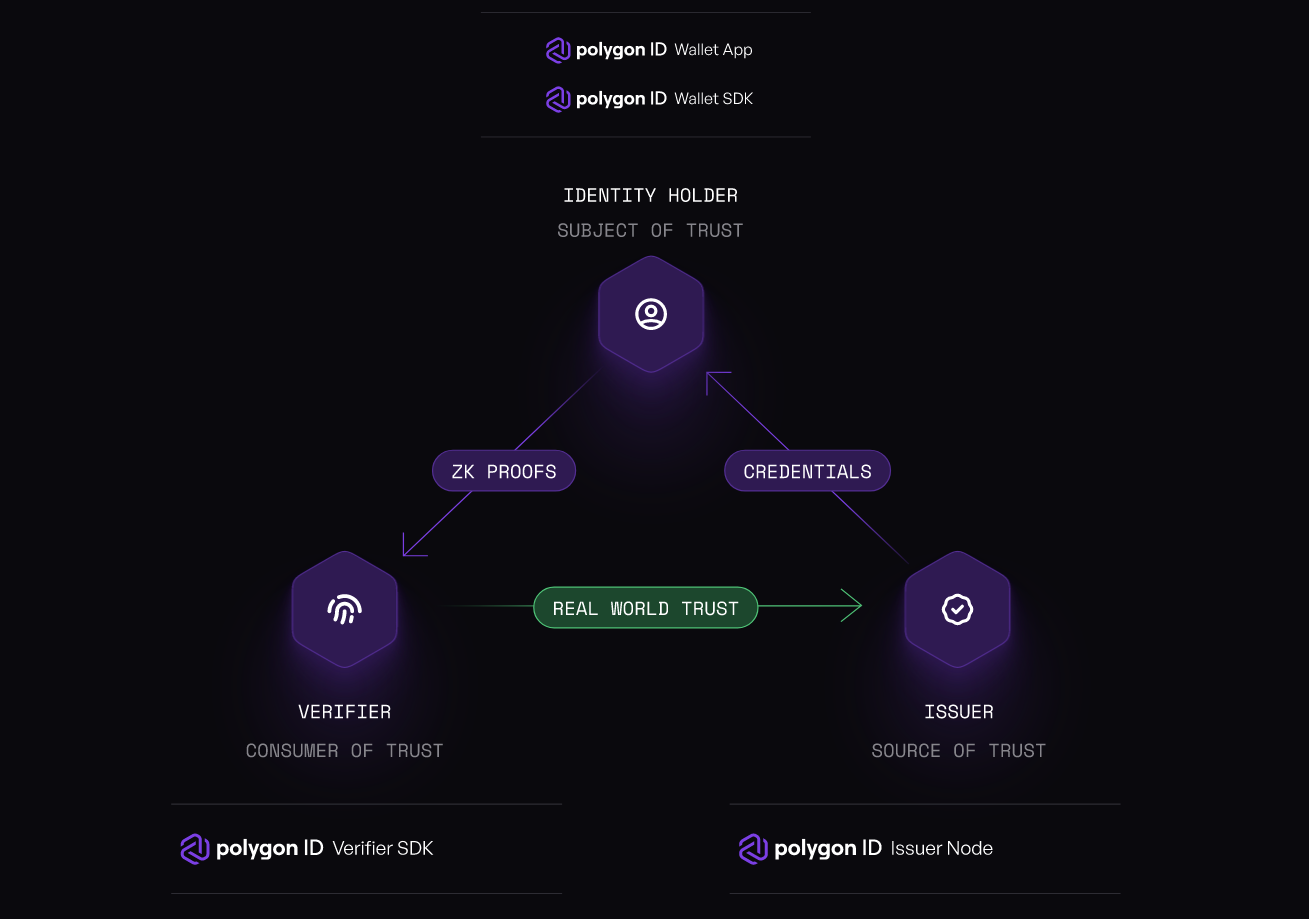
\includegraphics[scale=0.4]{media/polygonIddreieck}
	\caption{Zusammenspiel von Issuer, Holder und Verifier auf technischer Sicht in PolygonId \cite{ID31}}
	\label{fig:meine-grafik}
\end{figure}

Es ist zu erkennen, dass Polygon SDK's \footnote{Software Development Kits} für Entwickler zur Verfügung stellt um jeweils (Identity-) Holder, Verifier und Issuer zu implementieren. Für Wallets gibt es zudem eine Wallet-App. Für Issuer müssen Issuer Node gehostet werden, wodurch VC's ausgestellt oder entfernt werden können oder \textsl{Identity States} on-chain veröffentlicht werden können. Nach der Dokumentation \cite{ID38} muss der Node zusammen mit 

\begin{itemize}
	\item der Applikation
	\item einem 'Vault' für Key-Management-Services (Beispielsweise zum Speichern des privaten Schlüssels des Issuers)
	\item einem Cache-Service (Bespielsweise zum Zwischenspeichern von Templates, die einmalig von IPFS gedownloaded werden)
	\item einer Datenbank zum persistieren aller operativen Daten
\end{itemize}

Die Identitätsdaten bestehen aus folgenden drei Informationen, die jeweils in sog. 'Sparse Merkle Trees' gespeichert werden:
\begin{enumerate}
	\item \textbf{Claims Tree}: Ist ein Baum, der Informationen über ausgestellte Claims einer Identität \textbf{öffentlich} speichert.
	\item \textbf{Revocations Tree}: Ist ein Baum, der die Noncen (zuvor zufällig generierte Zahlen) einer Widerrufung von Claims \textbf{privat} speichert.
	\item \textbf{Roots Tree}: Speichert \textbf{öffentlich} die Historie der Wurzeln der Claim Trees.
\end{enumerate}
Der Identitätsstatus lässt sich somit wie folgt definieren:
\begin{align}
	IdState = Hash(ClR || ReR || RoR)
\end{align}
wobei:
\begin{itemize}
	\item Hash einer Hash-Funktion entspricht
	\item ClR der Wurzel des Claims Tree entspricht
	\item ReR der Wurzel des Revocation Tree entspricht
	\item ReR der Wurzel des Roots Tree entspricht
\end{itemize}
Der oben genannte Identitätsstatus wird als einziges Datum in der Blockchain gespeichert.

\subsection{zk-Proof von PolygonId}
Ein Feature von PolygonId, dass es von anderen SSI-Frameworks hervorhebt ist, dass es Verifikation mittels sog. \textsl{zero-knowledge-proofs} zur Verfügung stellt. Die Idee hierbei ist, dass dem Verifier die Richtigkeit eines Claims verifizieren kann \textbf{ohne} Informationen über den eigentlichen Claim zu erhalten. Als Beispiel wird folgender \textbf{nicht anonymisierter / nicht verschlüsselter/ selektiv freigegebener} Claim betrachtet:
\begin{lstlisting}[language=json,firstnumber=1]	
[...]
	"credentialSubject": {	
		"id": "did:example:456",	
		"degree": {		
			"type": "Gehalt",		
			"name": "ArbeitgeberName",		
			"frequence": "monthly",
			"value": 4000	
		}	
	}
[...]
\end{lstlisting}
Sollte nun beispielsweise ein Kreditinstitut (der Verifier) überprüfen wollen, ob der Kunde mehr als 2000€ verdient, so ist es in erster Linie irrelevant, ob die Person 5000€ oder 10000€ verdient und würde nur unnötig die Privatsphäre beeinträchtigen. Polygon bietet hierzu eine Lösung und implementiert ein zero-knowledge-Konzept, wo der Verifier über eine Query-Sprache lediglich über den Besitz des Credentials informiert wird ohne tatsächlich Informationen zu erhalten.
Die Anfrage kann on-chain und off-chain formuliert und sieht wie folgt aus (erstellt mit dem ZK-QueryBuilder\footnote{https://schema-builder.polygonid.me/query-builder} von PolygonId):

\begin{lstlisting}[language=json,firstnumber=1]	
[...]
    const proofRequest: protocol.ZKPRequest = {
		id: 1,
		circuitId: 'credentialAtomicQuerySigV2',
		query: {
			allowedIssuers: ['*'],
			type: 'EmployeeData',
			context: 'https://raw.githubusercontent.com/0xPolygonID/tutorial-examples/main/credential-schema/schemas-examples/employee-data/employee-data.jsonld',
			credentialSubject: {
				monthlySalary: {
					$gt: 2000,
				},
			},
		},
	};
[...]
\end{lstlisting}
Das Ergebnis der Anfrage ist ein Objekt, welches 'zero-knowledge-proof-information' speichert und dem Verifier zusichert, dass der zu verifizierende Nutzer den Claim tatsächlich besitzt.

\section{Sovrin}
\label{sovrin}
Sovrin (Foundation) \footnote{https://sovrin.org/} ist eine gemeinnützige Organisation, die etabliert wurde, um das Governance-Framework 'Sovrin Network' zu administrieren, welches ein öffentlicher Dienstleistungsservice ist zum ermöglichen der SSI \cite{ID39}. Dabei ist die Funktion der Sovrin Foundation das Sicherstellen des öffentlichen und global zugänglichen Sovrin-Identity-Systems.
Der verteilte Speicher des Netzwerks ist die eigen entwickelte Blockchain, die vollständig darauf abzielt SSI zu implementieren. Folgende vier Eigenschaften seien für ein erfolgreiches SSI-System notwendig und wurden in Sovrin Network eingebaut \cite{ID40}:
\begin{itemize}
	\item Governance: Alle Stakeholder können dem Netzwerk vollständig vertrauen
	\item Performance: Das Netzwerk soll auf dem gleichen Level skalieren wie das Internet selber
	\item Zugänglichkeit: Das Netzwerk ist für jeden zugänglich
	\item Privatsphäre: Die sichersten Standards werden implementiert
\end{itemize}
Ein Mechanismus zum verbessern der Privatsphäre ist das 'pseudonymous by default'-Konzept, welches Sovrin umsetzt. Hierbei wird für jede Relation (beispielsweise PersonX->Arbeitgeber, PersonX->Verkäufer, etc) eine eigene DID verwendet. Somit ist mehr Privatsphäre gegeben und auch die Sicherheit ist verbessert. \\
Die Sovrin-Blockchain ist eine sog 'permissioned' Blockchain, was bedeutet, dass ein Konten, der Transaktionen tätigen oder validieren möchte (also ein sog. 'Validator-Knoten') eine Erlaubnis braucht. Organisationen, die diese Erlaubnis erhalten haben nennen sich bei Sovrin 'Stewards'. Diese sind global verteilt und aktuell gibt es 50 Stewards in 13 Ländern und 6 Kontinenten \cite{ID43}. 
\subsection{Technische Grundlagen}
Sovrin versucht sich an DNS\footnote{Domain Name System} zu orientieren, da DNS knapp eine Milliarde Einträge hat und über 100 Milliarden anfragen pro Tag bearbeitet \cite{ID42}. Übertragen auf den Identitätskontext - unter der Annahme dass Identitäten mehrere DID's besitzten - muss das Netzwerk möglicherweise täglich Trillionen von Anfragen bearbeiten.
Während DNS keinen Konsensus-Algorithmus verwendet ist dies bei der Sovrin-Blockchain jedoch nicht der Fall. Um dennoch eine gute Skalierung zu implementieren werden zwei verschiedene Arten von Knoten im Netzwerk verwendet:
\begin{itemize}
	\item \textbf{Validator-Knoten}: Ist eine kleine Mengen an Knoten im Netzwerk deren Funktion es ist Transaktionen zu akzeptieren
	\item \textbf{Observer-Knoten}: Eine größere Menge an Knoten, die Lese-Anfragen bearbeiten
\end{itemize}
Issuer, Verifier und Holder erreichen diese Knoten über Agenten. Diese Agenden können beispielsweise Mobilanwendungen sein und haben die Aufgabe mit dem Sovrin-Network in Verbindung zu stehen. Agenten können Identitätstransaktionen stellvertretend für den Identitätsträger tätigen und kommunizieren direkt mit anderen Agenten. Dies funktioniert, da der Agent Zugriff auf den privaten Schlüssel hat. Demnach kann beispielsweise DID-Dokumente modifiziert werden oder Transaktionen getätigt werden.
Zudem werden private Daten (wie Claims) ebenso auf dem Agenten gespeichert, während öffentliche Daten auf der Blockchain abgelegt werden. \\
Ähnlich wie bei PolygonId kann von ZK-Proofs Gebrauch gemacht werden oder Anfragen modelliert werden.

\section{ShoCard}
Die letzte hier vorgestellte Lösung basiert auf der Bitcoin Blockchain. Das besondere hierbei ist, dass Bitcoin keine Möglichkeit bietet Smartcontracts oder ähnliches zu implementieren. Dennoch gibt es einen Prozess, der SSI in der Blockchain implementiert. Hierbei verschachtelt Shocard die DID, ein existierenden Credential und zusätzliche Identitätsattribute in einer Bitcoin-Transaktion \cite{ID46}. Shocard verwendet einen zentralen Server der folgende drei Vorgänge implementiert:

\begin{itemize}
	\item \textbf{Bootstrapping}: Ist der Prozess bei dem eine neue Shocard erstellt wird. Hierbei erstellt die Shocard-App ein neues asymmetrisches Schlüsselpaar und scannt die Credentials über die Kamera. Die Daten werden im Anschluss verschlüsselt und auf dem Gerät gespeichert. Ein signierter Hash wird im Anschluss in einer Bitcoin Transaktion gespeichert, wobei die erhaltene Transaktionsnummer zu der ShoCardID des Anwenders wird. Ebenso wird diese Information in der App gespeichert. Ist dieser Prozess abgeschlossen ,so kann der Identitätsträger mit mit Issuern kommunizieren, um weitere Identitätsattribute anzufragen. Dieser Prozess nennt sich certification
	\item \textbf{Certification}: Um Identitätsattribute zu erhalten muss der Identitätsträger nachweisen, dass er die Daten kennt, die den Hash generiert hatten (wurde in der App persistiert) und den Schlüssel der zur Signatur verwendet wurde. Als Ergebnis liegt eine neue Transaktion vor, die die Attribute und die ShoCardD gehasht enthält. Da der Provider die Transaktion getätigt hat, muss er die Transaktionsnummer zusammen mit dem signierten Klartext der neuen Attribute mit dem Nutzer teilen. Diese werden erneut in der Applikation lokal gespeichert. Da der Nutzer die Credentials jedoch nicht verlieren möchte im Falle, dass der Zugriff zur Applikation verloren geht, bietet ShoCard die Möglichkeit Credentials verschlüsselt in einem 'Envelop' zu speichern (ein Speicher den ShoCard verwaltet). Der Envelop kennt den Schlüssel zur Verschlüsselung nicht.
	\item Validation: Dieser Prozess findet statt, wenn ein Identitätsträger den Besitzt von Credentials nachweisen möchte. Hierbei gibt der Nutzer die Referenz des Envelops und den zur Verschlüsselung verwendeten Schlüssel. Somit kann der Verifier die Korrektheit überprüfen. Somit wird klar, dass kein ZK-Proof vorliegt, da dem Verifier sämtliche Informationen des Credentials vorliegen.	
\end{itemize}

\subsection{Probleme von ShoCard}
\label{shocard}
Mit der Verwendung von ShoCard gehen jedoch auch Probleme einher. Beispielsweise wird offensichtlich, dass wenn der \textbf{ShoCard central server} verwendet wird (der die Envelops speichert), dass eine Abhängigkeit zu ShoCard existiert. Sollte das Unternehmen verschwinden und die Server offline nehmen, so verlieren Nutzer ihren Zugang zu den Credentials, wenn sie keine lokale Kopie verwenden. Diese Eigenschaft nimmt ShoCard einen Teil seiner Dezentralität. Zudem existiert das Problem, dass ShoCardIDs nur unidirektional identifizieren (Also Identität -> ShoCardId). Es gibt keine dezentrale Registry, die von einer ShoCardID auf eine DID oder etwas Vergleichbarem auflöst. Zudem gibt es noch mehrere weitere Probleme \cite{ID46}.